\documentclass[12pt]{article}
%% arXiv paper template by Flip Tanedo
%% last updated: Dec 2016



%%%%%%%%%%%%%%%%%%%%%%%%%%%%%
%%%  THE USUAL PACKAGES  %%%%
%%%%%%%%%%%%%%%%%%%%%%%%%%%%%

\usepackage{amsmath}
\usepackage{amssymb}
\usepackage{amsfonts}
\usepackage{graphicx}
\usepackage{xcolor}
\usepackage{nopageno}
\usepackage{enumerate}
\usepackage{parskip}

%%%%%%%%%%%%%%%%%%%%%%%%%%%%%%%%%
%%%  UNUSUAL PACKAGES        %%%%
%%%  Uncomment as necessary. %%%%
%%%%%%%%%%%%%%%%%%%%%%%%%%%%%%%%%

\usepackage{tikzfeynman}

\usepackage{titlesec}
\titleformat*{\section}{\large\bfseries}

%% MATH AND PHYSICS SYMBOLS
%% ------------------------
%\usepackage{slashed}       % \slashed{k}
%\usepackage{mathrsfs}      % Weinberg-esque letters
%\usepackage{youngtab}	    % Young Tableaux
%\usepackage{pifont}        % check marks
\usepackage{bbm}           % \mathbbm{1} incomp. w/ XeLaTeX 
%\usepackage[normalem]{ulem} % for \sout


%% CONTENT FORMAT AND DESIGN (below for general formatting)
%% --------------------------------------------------------
\usepackage{lipsum}        % block of text (formatting test)
%\usepackage{color}         % \color{...}, colored text
%\usepackage{framed}        % boxed remarks
%\usepackage{subcaption}    % subfigures; subfig depreciated
%\usepackage{paralist}      % compactitem
%\usepackage{appendix}      % subappendices
%\usepackage{cite}          % group cites (conflict: collref)
%\usepackage{tocloft}       % Table of Contents	

%% TABLES IN LaTeX
%% ---------------
%\usepackage{booktabs}      % professional tables
%\usepackage{nicefrac}      % fractions in tables,
%\usepackage{multirow}      % multirow elements in a table
%\usepackage{arydshln} 	    % dashed lines in arrays

%% Other Packages and Notes
%% ------------------------
%\usepackage[font=small]{caption} % caption font is small



%\renewcommand{\thesection}{}
%\renewcommand{\thesubsection}{\arabic{subsection}}

%%%%%%%%%%%%%%%%%%%%%%%%%%%%%%%%%%%%%%%%%%%%%%%
%%%  PAGE FORMATTING and (RE)NEW COMMANDS  %%%%
%%%%%%%%%%%%%%%%%%%%%%%%%%%%%%%%%%%%%%%%%%%%%%%

\usepackage[margin=2cm]{geometry}   % reasonable margins

\graphicspath{{figures/}}	        % set directory for figures

% for capitalized things
\newcommand{\acro}[1]{\textsc{\MakeLowercase{#1}}}    

\numberwithin{equation}{section}    % set equation numbering
\renewcommand{\tilde}{\widetilde}   % tilde over characters
\renewcommand{\vec}[1]{\mathbf{#1}} % vectors are boldface

\newcommand{\dbar}{d\mkern-6mu\mathchar'26}    % for d/2pi
\newcommand{\ket}[1]{\left|#1\right\rangle}    % <#1|
\newcommand{\bra}[1]{\left\langle#1\right|}    % |#1>
\newcommand{\Xmark}{\text{\sffamily X}}        % cross out

% Change list spacing (instead of package paralist)
% from: http://en.wikibooks.org/wiki/LaTeX/List_Structures#Line_spacing
%\let\oldenumerate\enumerate
%\renewcommand{\enumerate}{
%  \oldenumerate
%  \setlength{\itemsep}{1pt}
%  \setlength{\parskip}{0pt}
%  \setlength{\parsep}{0pt}
%}

\let\olditemize\itemize
\renewcommand{\itemize}{
  \olditemize
  \setlength{\itemsep}{1pt}
  \setlength{\parskip}{0pt}
  \setlength{\parsep}{0pt}
}


% Commands for temporary comments
\newcommand{\comment}[2]{\textcolor{red}{[\textbf{#1} #2]}}
\newcommand{\flip}[1]{{\color{red} [\textbf{Flip}: {#1}]}}
\newcommand{\email}[1]{\texttt{\href{mailto:#1}{#1}}}

\newenvironment{institutions}[1][2em]{\begin{list}{}{\setlength\leftmargin{#1}\setlength\rightmargin{#1}}\item[]}{\end{list}}


\usepackage{fancyhdr}		% to put preprint number



% Commands for listings package
\usepackage{listings}      % \begin{lstlisting}, for code
%
 \lstset{basicstyle=\ttfamily\footnotesize,breaklines=true}
%    sets style to small true-type


%%%%%%%%%%%%%%%%%%%%%%%%%%%%%%%%%%%%%%%%%%%%%%
%%%  TIKZ COMMANDS FOR EXTERNAL DIAGRAMS  %%%%
%%%  requires -shell-escape               %%%%
%%%  in texpad 1.7: prefs > shell esc sec %%%%
%%%%%%%%%%%%%%%%%%%%%%%%%%%%%%%%%%%%%%%%%%%%%%

%% This is for exporting tikz figures as into a ./tikz/ subfolder.
%% It is useful if you want pdf versions of the tikz diagrams or
%% if you need to speed up compilation of a large document with
%% many tikz diagrams.

%\write18{} % Careful with this!
%\usetikzlibrary{external}
%\tikzexternalize[prefix=tikz/] % folder for external pdfs


%%%%%%%%%%%%%%%%%%%
%%%  HYPERREF  %%%%
%%%%%%%%%%%%%%%%%%%

%% This package has to be at the end; can lead to conflicts
\usepackage{microtype}
\usepackage[
	colorlinks=true,
	citecolor=black,
	linkcolor=black,
	urlcolor=green!50!black,
	hypertexnames=false]{hyperref}



%%%%%%%%%%%%%%%%%%%%%
%%%  TITLE DATA  %%%%
%%%%%%%%%%%%%%%%%%%%%

%%% PREPRINT NUMBER USING fancyhdr
%%% Don't forget to set \thispagestyle{firststyle}
%%% ----------------------------------------------
%\renewcommand{\headrulewidth}{0pt} % no separator
%\fancypagestyle{firststyle}{
%\rhead{\footnotesize \texttt{UCI-TR-2016-XX}}}



\begin{document}

%\thispagestyle{empty}
%\thispagestyle{firststyle} %% to include preprint

\begin{center}

    {\Large \textsc{Homework 5:} 
    \textbf{Complex Analysis}}


    
\end{center}

\vskip .4cm

\noindent
\begin{tabular*}{\textwidth}{rlcrll}
	\textsc{Course:}& Physics 231, \emph{Methods of Theoretical Physics} (2017)
	&
%	\hspace{1.2cm}
	&
	\\
	\textsc{Instructor:}& Flip Tanedo (\email{flip.tanedo@ucr.edu})
	&
	%\hfill
	&
	& 
	\\
	\textsc{Due by:}& Friday, November 3
	&
	%\hfill
	&
	%	
\end{tabular*}



\textbf{Reading}: For this week, continue last week's review of complex analysis. We will be using Fourier transforms, please brush up on these if you have forgotten the basic idea. Some possible references are the discussion around (5.57) of Byron and Fuller leading up to Chapter 5.7 or the section on Fourier transforms in Boas (Chapter 15.4 in the second edition). For our purposes, we'll just be using the $e^{ikx}$ basis of momentum space functions, not the trigonometric basis. 

We will have one lecture on dispersion relations, which you may want to review a a little ahead of time. That lecture will be outside of the main narrative of the course and you can also choose to appreciate it at a qualitative level. By the end of this week, you will be responsible for being able to calculate simple integrals using the residue theorem, so be sure review this in your favorite references. Boas does this reasonably well, but you may want to peek at a graduate level reference for a bit more detail.

We will have discussion section on Monday at 3:10pm in Chung 142. This is completely optional\footnote{For the record, lectures are also optional.}, but I welcome you to come to ask questions about the homework or the course at large. 




\section{A Green's function by patching}

\emph{This looks like a long problem, but it's mostly reading and understanding. Each step is modest.}

%\textcolor{blue}{\textbf{Correction} (10/27): The $(d/dx)^2$ operator is not self-adjoint. As we saw in class, the formally self adjoint operator is $-(d/dx)^2$. As a result, the eigenvalues of $(d/dx)^2$ are negative rather than positive. this problem has been updated to have the corrected operator. Homework 4 had the same error, though it only shows up in the plot for large $k^2$. Thanks to Wei-Xiang Feng for catching this.}

% This is kind of tricky, see page 270 of MW (9-4: inhomogeneous problems)

Thus far in this course, we have examined two ways of solving for Green's functions:
\begin{enumerate}
	\item \textbf{Fourier transform}. We talked about this briefly for the electrostatic problem. With this method, it is easy to solve for $\tilde G(k)$, the momentum space Green's function, but we will rely on the residue theorem to perform the integral to go back to position space.
	\item \textbf{Completeness and projection}. In Homework 4, Problem \#2 we solved a simple Green's function by using the completeness of a set of eigenfunctions. This method generalizes to the `named functions' of physics\footnote{For example: Bessel functions, Legendre polynomials, Spherical harmonics. To the best of my knowledge, `Spherical' was not a mathematician.} that are special because they are eigenfunctions for common classes of differential operators.
\end{enumerate}
In this problem we'll examine a third method based on patching together solutions of the homogeneous equation.  We examine the same system that you did in Homework 4, Problem \#2: consider a second order differential equation acting on a state $\psi(x)$ with a source $s(x)$. 
\begin{align*}
\mathcal O \psi(x) = 
	\left(-\frac{d^2}{dx^2} + k^2 \right) \psi(x) = s(x) \ .
\end{align*}
We consider the domain $x\in[0,1]$ with boundary conditions $\psi(0) = \psi(1) = 0$. \textbf{For simplicity}, we'll take $k^2 = 0$ and leave the $k^2 \neq 0$ case for extra credit.


%Matthews and Walker, p 258

We want to solve the Green's function equation, $$\mathcal O G(x,y) = \delta(x-y)\, .$$ In this method, we solve the \emph{homogeneous} equation $\mathcal O G(x,y) = 0$ for $x\neq y$ in the two regions $x<y$ and $x>y$. These two solutions will each have independent coefficients that we must patch together at $x=y$.

\subsection{Solve the homogeneous equation}

Solve the two \emph{homogeneous} equations in the regions away from the $\delta$-function spike:
\begin{align}
 	\left(\frac{d}{dx}\right)^2 G_{<}(x,y) = 0  
 	& \quad\text{ in }\quad 0 < x < y \leq 1 
 	\\
 	\left(\frac{d}{dx}\right)^2 G_{>}(x,y) = 0  
 	& \quad\text{ in }\quad 0 < y < x \leq 1
\end{align}
Don't forget to impose the boundary conditions $G(0, y) = G(L,y) = 0$. Understand why it makes sense that $\psi(0) = \psi(1) = 0$ imposes the same condition on the Green's functions. If the Green's function did not satisfy these conditions, then you could construct sources that violate the boundary conditions because $\psi(1) = \int G(1,y) s(y)\, dy \neq 0$.

The Green's function $G(x,y)$ is now piecewise defined
\begin{align}G(x,y) = \left\{ 
\begin{array}{ll}
 	G_<(x,y) & \quad\text{ if } x<y\\
 	G_>(x,y) & \quad\text{ if } x>y
 \end{array}\right. .
 \label{eq:piecewise:def}
 \end{align}
Check to make sure that you have the correct number of undetermined coefficients. 

\textsc{Hint}: if you're not sure what the solution to the homogeneous differential equation is, then you're over thinking it. It's not a trigonometric function. If you're still confused, refer back to your plot in Homework 4, Problem \#2.

\subsection{Patching, Part 1}
For fixed $y$, integrate the Green's function equation over an infinitesimal sliver, $x \in (y-\varepsilon, y + \varepsilon)$, with $\epsilon \to 0$: 
\begin{align}
	\int_{y-\varepsilon}^{y+\varepsilon} dx\, \left(\frac{d}{dx}\right)^2 G(x,y) &=  
	\int_{y-\varepsilon}^{y+\varepsilon} dx\; \delta(x-y)
	\ .
	\label{eq:patching:1}
\end{align}
\textsc{Hint}: It may be useful to remember that
\begin{align}
	\int_{y-\varepsilon}^{y+\varepsilon} dx\; \frac{df(x)}{dx} = f(y+\epsilon) - f(y-\epsilon) \ .
\end{align}

Write out the resulting equation in terms of $dG_</dx$ and $dG_>/dx$ at $x=y$. You will find that the slope of the Green's function, $dG/dx$, is \emph{discontinuous} at $x=y$. 


\subsection{Patching, Part 2}

Integrate (\ref{eq:patching:1}) again over $x\in(y-\epsilon y+\epsilon)$ to relate $G_<$ and $G_>$ at $x=y$.


\textsc{Answer}: $dG/dx$ has a finite discontinuity at $x=y$, therefore $G$ is \emph{continuous} at $x=y$. The discontinuity in the slope gives a kink in $G$,
\begin{align}
	\left.G_<(x, y)\right|_{x=y} &= \left.G_>(x, y)\right|_{x=y} \ .
\end{align}
We've found that the second derivative is a $\delta$-function (singular), the first derivative is simply discontinuous, and the zeroth derivative (the Green's function itself) is continuous.

\subsection{Patching, Part 3}

Take all of the above results and write down the piece-wise definition of $G(x,y)$ in (\ref{eq:piecewise:def}) as an explicit function of $x$ and $y$ with all coefficients determined. Sketch $G(x,y)$  for $y=0.5$ and compare it to your plot from Homework 4, Problem \#2.

\subsection{Extra Credit: $k^2\neq 0$}

\emph{This problem is not graded and is purely for your ``enjoyment.''} Perform the same steps for the case of $k^2\neq 0$. The homogeneous solution is now a sine, which makes things a bit more complicated. The procedure is completely the same and the $k^2 \lesssim 1$ case is well approximated by $k^2=0$, as you will have noticed from the plot in Homework 4, Problem \#2. \textsc{Solution}: Matthews \& Walker, Chapter 9--4. 

\section{Practice with complex integration}
% Boas 14.3.1

\subsection{This is not a closed loop}

The goal of this problem is to review line integrals in a 2D space. Perform the integral
\begin{align}
	\int_i^{1+i} dz \; z \,
\end{align}
with respect to the path that connects $z=i$ and $z=i+1$ by a straight line segment. This is \emph{not} a closed loop, there's no magic formula for this. Just parameterize the path by writing $z$ as a function of a real parameter. Then write out $dz$ in terms of the parameter. Do the integral.

\subsection{Contour integrals}

Calculate the following integrals using the residue theorem:
\begin{enumerate}[(a)]
	\item $\displaystyle \int_{0}^\infty \frac{x^2}{x^4 + 16} dx$ % Boas ch 7 probs
	\item $\displaystyle \int_{-\infty}^\infty \frac{\sin x}{x^2 + 4x + 5}dx$ % Boas ch 7 probs
	\item $\displaystyle \int_{0}^\infty \frac{1}{x^6+1}dx$ using a contour including the real line and a large semicircle in the complex plane % Appel ch 4 probs
	\item $\displaystyle \int_{0}^\infty \frac{1}{x^6+1}dx$ using a contour that encloses the `pizza slice' wedge between $\theta = 0$ and $\theta = \pi/3$. 
\end{enumerate}

\textsc{Hint}: for (d), the line integral along the diagonal is proportional to the integral you want. % Appel ch 4 probs


%
%\section{Cauchy--Riemann in silly coordinates}
%
%% From ComplexIntegration.pdf
%% http://link.springer.com/chapter/10.1007%2F978-3-319-00212-5_1#Sec23
%% solutions in the back
%
%\begin{enumerate}[(a)]
%	\item Write the Cauchy--Riemann equations in polar coordinates.
%\begin{align}
%	f(z) = f(r,\theta) = u(r,\theta) + i v(r,\theta) \, .
%\end{align}
%\textsc{Hint}: you want $\Delta f/\Delta z$ as $\Delta z \to 0$. Unlike the Cartesian case, you cannot just take $\delta z$ along the $\Delta \theta$ direction because that doesn't correspond to $\Delta z \to 0$ by itself.
%%
%\item Show that $f(z) = \ln z$ is analytic for all finite (nonzero) $z$.
%\end{enumerate}
%

%\section{Cauchy's Integral Formula for derivatives}
% Boas 5.2

\section{How to find Residues}

% Boas p. 599, Appel 4.5d
We saw that a \textbf{meromorphic} (analytic up to poles) function has a Laurent series expansion about a point $z_0$,
\begin{align}
f(z) &= \sum_{n=-\infty}^{\infty} a_n (z-z_0)^n
	\ .
\end{align}
The $a_{-1}$ term has special significance and is known as the \textbf{residue} of $f$ at $z_0$, $\text{Res}(f,z_0)$. When we have an explicit Laurent expansion about $z_0$, identifying the residue is a matter of reading off the $(z-z_0)^{-1}$ coefficient. Alternately, when $z_0$ is a simple pole the function can be written as
\begin{align}
	f(z) = \frac{F(z)}{(z-z_0)} \ ,
\end{align}
where $F(z)$ is analytic at $z_0$. In this case, the residue is $\text{Res}(f,z_0) = F(z_0)$. This leads to the sometimes useful guide: If $f(z_0)$ is not finite but $(z-z_0)\, f(z)$ is finite, then
	\begin{align}
		\text{Res}(f,z_0) &=  \lim_{z\to z_0} (z-z_0)\, f(z) \ .
	\end{align}
What do we do if $(z-z_0)\, f(z)$ is \emph{not} finite? For example, what if both $a_{-1}$ and $a_{-2}$ were non-zero? How does determine the residue ($a_1$) in such a case? Explain why the following algorithm works: Find the positive integer $m$ such that $F_m(z)=(z-z_0)^m f(z)$ is finite at $z=z_0$, then the residue is
\begin{align}
	\text{Res}(f,z_0) = \left.\frac{1}{(m-1)!} \frac{d^{m-1}}{dz^{m-1}} F_m(z)\right|_{z=z_0} \ .
\end{align}

\textsc{Hint}: We did in Lecture 13 for the case of a second-order pole. This problem asks you to generalize the residue to the case of an $m^\text{th}$ order pole.

\textsc{Hint}: The proof doesn't have to be rigorous. And if you're struggling where to start, review our examination of the case $m=2$. Then see what happens for $m=3$. Proceed until you see the pattern.


\appendix
\section*{\Large Extra Credit}


These problems are not graded and are for your edification. You are strongly encouraged to explore and discuss these topics, especially if they are in a field of interest to you.


\section{Laurent Theorem}

We shall prove the Laurent Theorem for the expansion about $z_0$ of a function $f(z)$ in a region where it is meromorphic:
\begin{align}
f(z) &= \sum_{n=-\infty}^{\infty} a_n (z-z_0)^n
&
a_n &= \frac{1}{2\pi i} \oint_C \frac{f(z)}{(z-z_0)} dz \ ,
\end{align}
where $C$ is a contour that loops once counter-clockwise around $z_0$.

Consider the contour below (image from Cahill, \emph{Physical Mathematics}), enclosing an annular region that includes the point $z$ without any poles (asterisks).
\begin{center}
% Image from Cahill, Fig 5.5
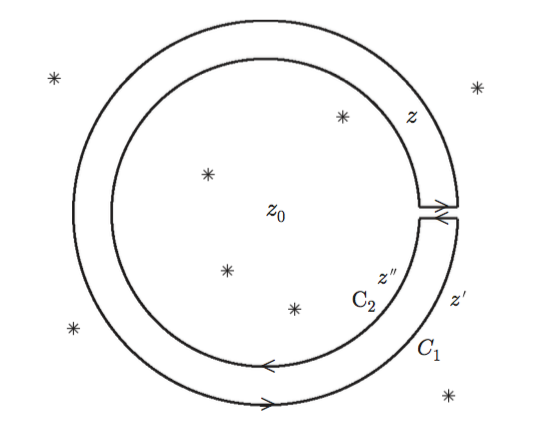
\includegraphics[width=.5\textwidth]{Cahill_5_5}
\end{center}
Both the outer and inner contours, $C_1$ and $C_2$, encircle $z_0$. Use the \textbf{Cauchy theorem},
\begin{align}
	f(z) = \frac{1}{2\pi i} \oint_{C} \frac{f(w)}{w-z_0} dw \ ,
	\label{eq:laurent}
\end{align}
where $C$ encloses a region in which $f(z)$ is \emph{analytic}. Taking $C = C_1 - C_2$, the contour shown above, one has
\begin{align}
	f(z) = 
	\frac{1}{2\pi i} \oint_{C_1} \frac{f(z')}{z'-z} dz'
	-
	\frac{1}{2\pi i} \oint_{C_2} \frac{f(z'')}{z''-z} dz'' \ .
	\label{eq:laurent:int}
\end{align}
Consider the following quantities:
\begin{align}
	r(z') &= \frac{z-z_0}{z'-z_0}
	&
	R(z'') &= \frac{z - z_0}{z''-z_0} \ .
\end{align}
Note that $|r(z)| < 1$ and $|1/R(z)| < 1$. Write (\ref{eq:laurent:int}) as
\begin{align}
	f(z) = 
	\frac{1}{2\pi i} \oint_{C_1} \frac{f(z')}{(z'-z_0)\left[1-r(z')\right]} dz'
	-
	\frac{1}{2\pi i} \oint_{C_2} \frac{f(z'')}{(z-z_0)\left[1-1/R(z'')\right]} dz'' \ .
\end{align}
Use the series expansion
\begin{align}
	\frac{1}{1-s} = \sum_{n=0}^\infty s^n \ ,
\end{align}
for $|s|<1$. Argue that we may now deform $C_1$ and $C_2$ to an intermediate contour $C$. Show that the result of all this proves (\ref{eq:laurent}).




\end{document}